\section{Validation and measured performance}\label{sec:experiments}

\subsection{Correctness checks and what they establish}

The complete integrated suite passed \textbf{254 test methods}, with zero
failures or errors, in 36.700 seconds on Python 3.12.14. Of these, 209
are inherited methods and 45 belong to the four new test modules.
The execution log and a machine-readable summary are included.
Many methods contain whole finite enumerations, so a test-method count
is not the number of individual algebraic comparisons.

\begin{center}
\small
\begin{tabular}{p{0.29\linewidth}p{0.62\linewidth}}
\toprule
Check & Coverage\\
\midrule
Tail module, 11 methods &
400 seeded complete-profile comparisons with the macro backend;
80 comparisons with the independently assembled crossing cube;
both signs, arbitrary selected positions, threshold endpoints, links,
original parity, resource failure, and enormous exponents.\\
Streaming module, 17 methods &
468 exhaustive signed words against the independent cube, plus six
dedicated examples; all compact map types, degree and boundary ranks,
cache caps, differential-square checks, live-state counts, and early
decision semantics.\\
Structural module, 8 methods &
3,026 exhaustive checked source-versus-PD summaries; 240 higher-strand
seeded pipeline comparisons; signature domination, path optimization,
invalid inputs, and 100,001-bit exponent arithmetic.\\
Continuation interface, 9 methods &
All three exact backends, structural-first recognition, complete link
homology, original component checks, resource \code{UNKNOWN}, stdin,
configuration errors, and exit codes.\\
Separate recurrence audit &
104 contexts and 208 signed families; 832 macro and 220 independent
crossing-cube comparisons, without calling the tail implementation.\\
Separate slope audit &
500 comparisons of the central-matrix slope with ordinary reduced
homology of the extracted turnback-context complex.\\
\bottomrule
\end{tabular}
\end{center}

The exhaustive word sets include equivalent words, repeated knot types,
links, and empty words; they are not catalogues of distinct knots.
The independent crossing cube does not use the run recurrence or
its local compression, which makes it a meaningful implementation
cross-check. It still shares the characteristic-two Frobenius theory
and some representation conventions. Neither repeated implementations
nor finite tests are substitutes for the mathematical proof.

Two large-encoding checks illustrate the exact scope. For both signs,
a two-strand exponent \(m=2^{100000}+1\), having 100,001 bits, is
handled from a four-element reference basis. The result has two
exceptional degrees and one interval, and its exact rank is \(m\).
For
\[
\sigma_1^3\sigma_2^{-3}\sigma_3^{\,10^{100}+1}
\quad\text{on four strands},
\]
the returned rank is \(9(10^{100}+1)\), the slope is \(9\), and the
reference basis has fewer than 1,000 elements.
These checks exercise big-integer arithmetic and avoid exponent
expansion; they do not certify that a reference of arbitrary context
size will fit the resource budget.

\begin{figure}[htbp]
\centering
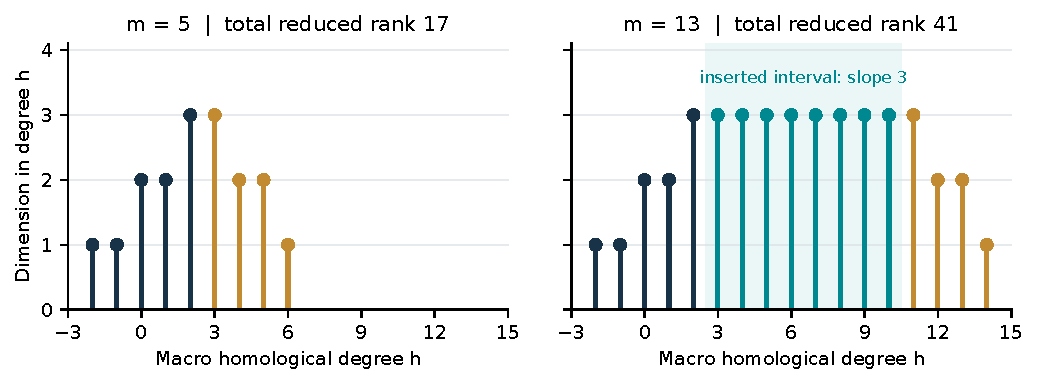
\includegraphics[width=\linewidth]{figures/exact_profile.pdf}
\caption{Exact reduced homological profiles of
\(\sigma_1^m\sigma_2^{-1}\sigma_1\sigma_2^{-1}\).
The dark lower region is fixed, the gold upper region translates by
\(m-5\), and the teal interval contributes rank \(3\) in each inserted
degree. Both panels are generated from exact output; the recurrence is
proved independently of the plotted examples.}
\label{fig:profile}
\end{figure}

\subsection{Paired long-run homology measurements}

The recurrence benchmark uses seven A/B/A rounds per case, a separate
seven-pair A/A control, and fresh computation caches. A is the ordinary
macro backend; B is the exact recurrence. A returns an explicit degree
dictionary and B an exact compressed profile. Their complete homological
information agrees. Expansion of B's compact interval is excluded from
its timed task, because compact output is the interface whose complexity
is being measured.

The benchmark contains three families at selected lengths
\(17,65,257,1025\), plus a below-threshold no-compression control.
There is no braid simplification or earlier recognition filter in these
timings. The three largest-length results are:

\begin{center}
\small
\begin{tabular}{lrrrrr}
\toprule
Family, \(m=1025\) & \(\N(m)\) & \(\N_0\) &
A (ms) & B (ms) & Paired A/B\\
\midrule
Two strands & 1,027 & 4 & 3.639 & 0.084 & 39.42\\
Figure-eight context & 15,393 & 93 & 44.000 & 0.637 & 69.12\\
Mixed four-strand link & 18,486 & 126 & 37.998 & 0.931 & 44.05\\
\bottomrule
\end{tabular}
\end{center}

Durations are medians, with A averaged over the two surrounding calls in
each round. The final column is the median of the paired round ratios,
not the quotient of the separately displayed medians.
The mixed four-strand input is
\(\sigma_1^m\sigma_2^{-1}\sigma_3\sigma_2^{-1}\);
its measured odd-\(m\) closure is a link, and the benchmark computes its
marked reduced homology.

The no-compression control had median A/B \(1.021\), with individual
ratios from \(0.723\) to \(1.355\). The separate A/A control had median
second/first \(1.064\). Small durations are visibly noisy.
The algebraic count reduction, the exact equality checks, and the
asymptotic theorem are stronger evidence than a single microbenchmark
ratio. These are standalone full-homology gains. By
\cref{cor:dominant}, the knot families in the proved long-run range are
already structurally decided by the baseline.

\begin{figure}[htbp]
\centering
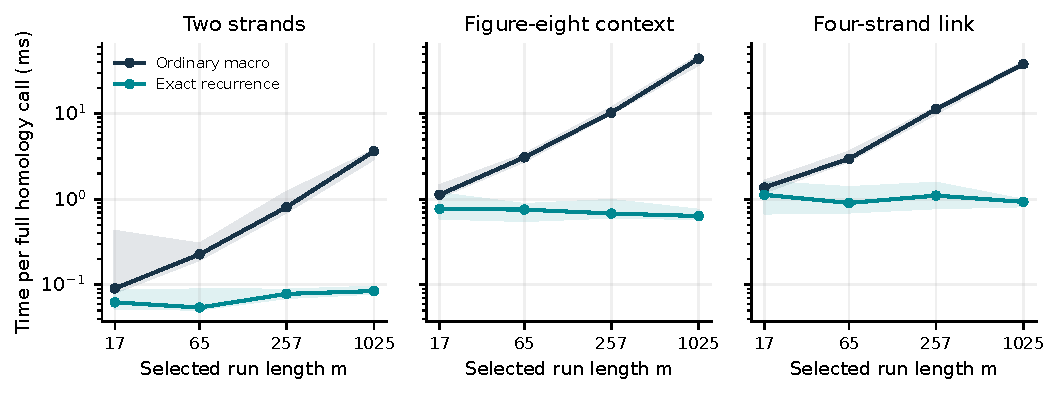
\includegraphics[width=\linewidth]{figures/tail_scaling.pdf}
\caption{Median standalone homology times at four run lengths.
Shading shows the interquartile ranges of the retained paired samples.
Both axes are logarithmic. The finite reference is unchanged within each
family; the measurements still show ordinary host and timing variability.}
\label{fig:tailtimes}
\end{figure}

\subsection{Streaming: memory savings with an observed time cost}

The streaming experiment uses eight cases and seven randomized rounds,
with five fresh calls per arm per round. Each round includes an
identical original-backend control. Full ranks, homological profiles,
chain dimensions, and boundary ranks are compared. Differential-square
checking occurs before timing. Memory tracing occurs in separate fresh
runs, so its instrumentation does not contaminate the duration
measurements.

Across these cases, the paired original/streamed time ratios range from
\(0.265\) to \(0.698\): complete streamed homology is slower.
The original/streamed peak traced-allocation ratios range from
\(1.028\) to \(3.064\): peak allocation is smaller.
A/A time ratios range from \(0.849\) to \(1.198\).
The allocation measurements are newly traced Python allocations from
\code{tracemalloc}, not process RSS or a hardware memory lower bound.

\begin{figure}[htbp]
\centering
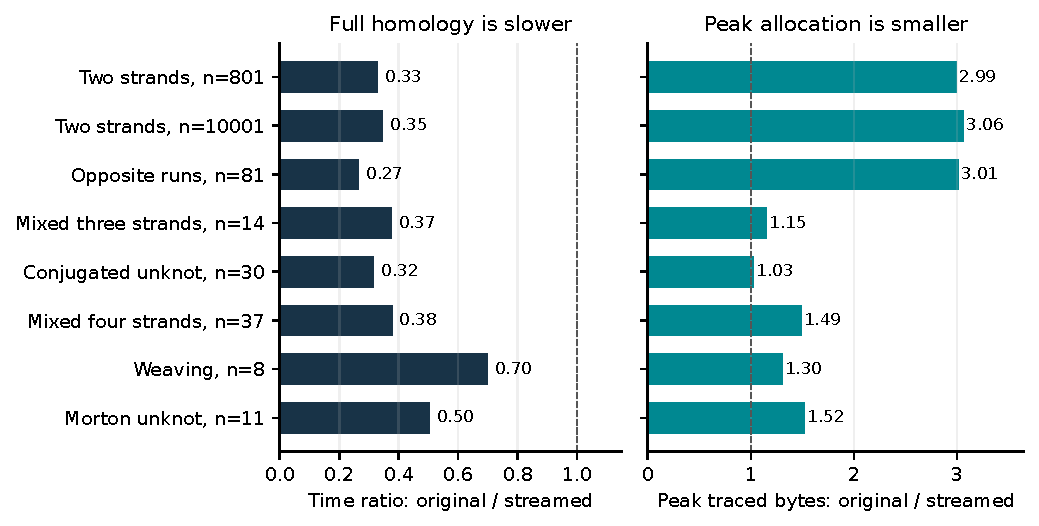
\includegraphics[width=\linewidth]{figures/streaming_tradeoff.pdf}
\caption{The full-homology time--space tradeoff across all eight streamed
benchmark cases. A ratio below one on the left means the streamed
implementation is slower. A ratio above one on the right means it uses
fewer peak traced bytes. The dashed line is equality.}
\label{fig:streamtradeoff}
\end{figure}

The repository's actual Morton input is an informative complete
unknot example:
\[
[-3,-3,2,-3,2,1,1,1,-2,1,-2]\quad(b=4).
\]
It has 768 macro states and 2,799 reduced basis elements.
In degrees \(-5,\ldots,6\), its chain dimensions and outgoing ranks are
\[
\begin{array}{r|rrrrrrrrrrrr}
h&-5&-4&-3&-2&-1&0&1&2&3&4&5&6\\ \hline
d_h&8&48&138&270&417&518&510&414&278&142&48&8\\
r_h&8&40&98&172&245&272&238&176&102&40&8&0
\end{array}
\]
so \eqref{eq:betti} gives one class in degree zero and no others.
The streamed run retains at most 308 state entries and 272 pivots.
The dense full-matrix sum is \(Q=1{,}009{,}952\) bits; the ordinary
streamed live envelope is 140,760 bits.
These are two structural bounds, not measured byte values.

The measured Morton medians are 27.360 ms for the original and
50.385 ms for streaming. Peak traced allocations are 1,441,224 and
946,172 bytes, respectively, a \(1.523\)-fold reduction.
Thus the implementation improves memory use on an actual full-rank-one
calculation but does not justify replacing the faster default on
time grounds.

For \(\sigma_1^{10001}\), full original and streamed computations take
37.742 and 100.604 ms, while streamed early recognition takes 0.118 ms
and visits four states. The four-strand mixed case of 37 crossings
visits 192 of 2,048 states before an early lower bound exceeds one.
These demonstrate the correctness and possible value of an early
backend endpoint. They do not measure its value after the existing
structural and modular filters.

\subsection{Separating encoding savings from recognition savings}

The structural experiment uses
\[
\gamma_m=\sigma_1^m\sigma_2^{-(2m-1)}\sigma_3^m,\qquad
b=4,\quad m\ge3\text{ odd}.
\]
These are one-component homogeneous braids with exponent sum \(1\),
zero Rasmussen interval, and positive canonical genus.
The homogeneous-genus criterion already proves nontriviality.
The coarse exponent-sum obstruction alone does not do so.

One experiment times a direct RLE certificate against expansion of
the word, checked PD construction, and the existing Seifert certificate.
A second uses fresh prebuilt diagrams and changes only the opt-in
\code{use_braid_profile} argument to the recognizer; construction is
outside that second timer.

\begin{center}
\small
\begin{tabular}{rrrrr}
\toprule
\(m\) & Crossings & Expanded construction / RLE &
Profile off / on & Pipeline A/A\\
\midrule
17 & 67 & 107.71 & 2.76 & 0.964\\
129 & 515 & 999.73 & 4.49 & 1.168\\
1025 & 4099 & 6645.13 & 4.03 & 1.039\\
4097 & 16387 & 36063.64 & 3.48 & 0.884\\
\bottomrule
\end{tabular}
\end{center}

All ratios are medians of paired rounds. The large construction-inclusive
ratios measure the explicit encoding difference: three integer runs
versus thousands of crossings and PD incidences. They are not general
recognition speedups. The prebuilt-diagram experiment shows an additional
constant-factor improvement on these selected structural cases.
All decisions and all compared Seifert metadata agree.
The Morton structural-only control remains \code{INCONCLUSIVE} in
both implementations; its full recognizer is excluded from that
experiment.

The first shorter batches showed substantial timer noise. Both pilot
files are retained, and the final script uses fixed size-based larger
batches rather than selecting favorable samples.
The reported A/A controls still require approximate interpretation.
The polynomial encoded-input theorem is independent of those timings.
